\documentclass[10pt,a4paper]{article}
\usepackage[utf8]{inputenc}
\usepackage{amsmath}
\usepackage{amsfonts}
\usepackage{amssymb}
\usepackage{german}
\usepackage{fancyhdr}
\usepackage{graphicx}
\usepackage[german]{babel}
\renewcommand{\listfigurename}{Test}
\usepackage{geometry}
\usepackage{listings}
\usepackage{hyperref}
\usepackage[onehalfspacing]{setspace}
\usepackage{color}
\usepackage[usenames,dvipsnames]{xcolor}
\usepackage{DejaVuSans}
\usepackage[T1]{fontenc}
\usepackage{amsmath}
\usepackage{float}

\renewcommand*{\familydefault}{\sfdefault}
\geometry{verbose,a4paper,tmargin=35mm,bmargin=35mm,lmargin=25mm,rmargin=25mm}
\author{Dominik Heeb, Fabian Keller}
\title{Dynamic Paralle Checker}
\pagestyle{fancy}
\fancyhead{}
\fancyhead[L]{Dynamic Paralle Checker}
\fancyhead[R]{Domink Heeb, Fabian Keller}
\fancyfoot{}
\fancyfoot[R]{Seite \thepage}
\definecolor{backcolor}{rgb}{0.95,0.95,0.92}
\definecolor{bluekeywords}{rgb}{0,0,1}
\definecolor{greencomments}{rgb}{0,0.5,0}
\definecolor{redstrings}{rgb}{0.64,0.08,0.08}
\definecolor{xmlcomments}{rgb}{0.5,0.5,0.5}
\definecolor{types}{rgb}{0.17,0.57,0.68}
\lstset{language=[Sharp]C,
captionpos=b,
showspaces=false,
showtabs=false,
breaklines=true,
showstringspaces=false,
breakatwhitespace=true,
escapeinside={(*@}{@*)},
commentstyle=\color{greencomments},
morekeywords={partial, var, value, get, set},
keywordstyle=\color{bluekeywords},
stringstyle=\color{redstrings},
basicstyle=\ttfamily\normalsize,}

\usepackage{amsmath}
\usepackage[some]{background}
\usepackage{lipsum}

\definecolor{titlepagecolor}{cmyk}{1,.20,0,.25}

\DeclareFixedFont{\bigsf}{T1}{phv}{b}{n}{1.5cm}

\backgroundsetup{
scale=1,
angle=0,
opacity=1,
contents={\begin{tikzpicture}[remember picture,overlay]
 \path [fill=titlepagecolor] (-0.5\paperwidth,5) rectangle (0.5\paperwidth,10);  
\end{tikzpicture}}
}
\makeatletter                       
\def\printauthor{%                  
    {\LARGE Studenten:\\\vspace{10pt}
    \large \@author \\\vspace{20pt}
    \LARGE Dozent:\\\vspace{10pt}
    \large Prof. Dr. Luc Bläser \\
	\texttt{lblaeser@hsr.ch}}}            
\makeatother
\author{%
    Fabian Keller \\
    Semester 5 \\
    \texttt{f3keller@hsr.ch}\vspace{15pt} \\
    Dominik Heeb \\
    Semester 5 \\
    \texttt{d1heeb@hsr.ch}
    }

\begin{document}
\begin{titlepage}
\BgThispage
\newgeometry{left=1cm,right=4cm}
\vspace*{2cm}
\noindent
\textcolor{white}{\bigsf Dynamic Parallel Checker\\[0.5cm] \begin{huge}Semesterarbeit - Technische Dokumentation\end{huge}}
\vspace*{2.0cm}\par
\noindent
\begin{minipage}{0.35\linewidth}
    \begin{flushright}
        \printauthor
    \end{flushright}
\end{minipage} \hspace{15pt}
%
\begin{minipage}{0.02\linewidth}
    \rule{1pt}{300pt}
\end{minipage} \hspace{40pt}
%
\begin{minipage}{0.6\linewidth}
\begin{center}
\begin{huge}
Eine Studie über Dynamic Parallel Checking Methoden
\end{huge}
\end{center}
\end{minipage}
\end{titlepage}
\restoregeometry

\newpage
\tableofcontents 
\newpage

\section{Abstract}
\begin{flushleft}
In diesem Projekt werden verschiedene Methoden zur dynamischen Analyse von Parallelem Code evaluiert. Dafür wird ein Dynamic Parallel Checker Prototyp entwickelt, der während der Laufzeit überprüft ob Nebenläufigkeitsfehler (Race Conditions) auftreten. Ebenfalls Inhalt dieses Projekts ist es, einen eigenen Algorithmus zu entwickeln, der die Laufzeitanalyse ermöglicht. Diesbezüglich haben wir uns für einen Algorithmus entschieden, der mit Hilfe einer Vector Clock eine partielle Ordnung innerhalb der Lese- und Schreibzugriffe von den verschiedenen Threads herstellen kann.\\
Um eine Applikation zu überwachen wird der Microsoft Intermediate Language Code der Applikation mit Hilfe des Frameworks Mono.Cecil instrumentiert. Dabei werden nur die Operation Codes instrumentiert, die einen Lese- oder Schreizugriff durchführen, oder mit der Synchronisation zwischen zwei Threads oder Tasks zu tun haben.\\
Im Rahmen unseres Projektes haben wir uns auf einen gewissen Umfang der Instrumentierung beschränkt, dazu mehr im Kapitel \ref{implementation} Implementation.\\
Die Erkennung von Race Conditions findet innerhalb unserer eigenen Dynamic Parallel Checker Library statt. Damit diese Library die benötigten Informationen erhält, wann welcher Thread einen Lese- oder Schreibzugriff auf welche Ressource durchgeführt hat, fügen wir bei den relevanten Operation Codes des IL Codes einen Aufruf auf unsere Library hinzu. 
Diesem Aufruf übergeben wir die Referenz zu der Ressource, auf die zugegriffen wurde, die Zeilennummer des IL Codes und den Methodennamen, in dem der Zugriff stattgefunden hat. In der Library wird für jeden Thread oder Task eine eigene History der Lese- und Schreibzugriffe mitgeführt. Diese Informationen werden verwendet um die neben läufigen Zugriffe zu identifizieren und um dann zu überprüfen, ob eine Race Condition auftrat. Zusätzlich zu der Zugriffs-History wird auch noch eine Lock-History geführt, die es erlaubt eine Synchronisation zwischen zwei Threads oder Tasks , die durch einen Lock zwingend sequenziell abgelaufen sind, durchzuführen. Mehr dazu im Kapitel \ref{lock_history} Lock-History.\\
Unser Projekt beinhaltet ebenfalls eine WPF Applikation, die es ermöglicht unsere Library zu nutzen. Unsere DPC Library meldet alle Race Conditions an diese Applikation und stellt diese in einer Liste dar. Als kleines Zusatzfeature für die Erleichterung der Fehlersuche dekompilieren wir den Code der betroffenen Methoden und stellen diesen ebenfalls dar.\\
\end{flushleft}
\newpage
\section{Technischer Bericht}
\subsection{Einleitung und Übersicht}
Dieses Kapitel beinhaltet eine Beschreibung der verwendeten Konzepte und Technologien dieses Projekts. Für das Verständnis des gesamten technischen Berichts empfehlen wir das Lesen dieses Teils. Bei bereits vorhandener Fachkenntnis bezüglich der Thematik kann dieser Teil gerne übersprungen werden und direkt die Implementation betrachtet werden.
\subsubsection{Dynamic Checker}
\begin{flushleft}
Um Race Conditions (sh. \ref{race_conditons}) zu erkennen, gibt es verschiedene Ansätze. Zwei davon sind, der Dynamic Checker und der Static Checker. In diesem Projekt
wird ein Dynamic Checker entwickelt. Ein dynamic Checker hat die Aufgabe, Race Conditions zur Laufzeit (dynamic) zu erkennen. Der Static Checker
im Gegensatz behandelt das Erkennen zur Entwicklungszeit. Um einen Dynamic Checker realisieren zu können, muss ein fertiges Programm instrumentiert werden.
Mit Instrumentation ist gemeint, dass der Kompilierte Code angepasst wird, so dass er während der Laufzeit einen Erkennungsalgorithmus ausführen kann, jedoch nicht das Verhalten des Programms verändert.\\
Der Checker analysiert hauptsächlich Lese- und Schreibzugriffe auf Variablen. Um die Präzision zu erhöhen, müssen auch Lock/ Unlock und Thread.Start usw. ausgelesen werden.\\
Mehr informationen dazu unter: \ref{vector_algorithm} Vector Clock Algorithmus
\end{flushleft}
\subsubsection{Race Condition}\label{race_conditons}
\begin{flushleft}
Bei Race Conditions handelt es sich um Speicherzugriffsfehler. Diese können durch richtige synchronisation (Codeteile, in welchen nur ein Thread gleichzeitig arbeiten kann) verhindert werden. In \autoref{fig:exampleRaceCondition} wird ein Code beschrieben, welcher diese Synchronisation komplett weglässt und daher Race Conditions entstehen.
\begin{figure}[H]
\centering
\begin{tabular}{|cc|}
\hline
\multicolumn{2}{|c|}{Konto = 100} \\ 
 &  \\ 
Thread 1 & Thread 2 \\ 
Konto + 200 & Konto - 100 \\ 
\hline
\end{tabular}
\caption[Beispiel Race Condition]{Ein unsynchronisierter Zugriff auf ein Konto}
\label{fig:exampleRaceCondition}
\end{figure}
Wenn zwei Threads den Code unter \autoref{fig:exampleRaceCondition} parallel ausführen, ist nicht deterministisch welcher Thread wann durchgeführt wird. Die Situation in \autoref{fig:exampleRaceCondition2} kann dadurch entstehen. Dabei erfährt der zweite Thread nicht, das der erste Thread den Wert angepasst hat und überschreibt den Wert mit seinen falschen Daten.\\\newpage
\begin{figure}[H]
\centering
\begin{tabular}{|cc|}
\hline
Thread 1 & Thread 2\\
Lesen Konto = 100 & \\
& Lesen Konto = 100\\
Addieren 100 + 200 & Addieren 100 - 100\\
Speichern 300 &\\
& Speichern 0\\
\multicolumn{2}{|c|}{Konto = 0}\\
\hline
\end{tabular}
\caption[Race Condition]{Ablauf eines unnsynchronisierten Zugriff}
\label{fig:exampleRaceCondition2}
\end{figure}
Race Conditions wie unter \autoref{fig:exampleRaceCondition2} sind gefährlich, da kein effektiver Fehlzustand im System ensteht, sondern Werte nicht richtig angepasst werden. Race Conditions zeichnen sich auch daher aus, dass sie stark vom Verarbeitungsablauf abhängen und daher nicht immer auftreten müssen. Wenn also die Threads in \autoref{fig:exampleRaceCondition2} in der richtigen Reihenfolge verarbeitet werden, wird kein Fehler entstehen.\\

\end{flushleft}
\subsubsection{Vector Clock}
\begin{flushleft}
Die einzelnen Lese- und Schreibzugriffe in einem System können asynchron in unterschiedlichen Threads ablaufen und dadurch nicht in eine totale Ordnung gebracht werden. Um nun jedem einzelnen Zugriff einen Zeitstempel zuzuordnen verwenden wir eine Vector Clock. Diese Vector Clock wird benötigt um eine Aussage über die Nebenläufigkeit der einzelnen Zugriffe zu machen.\\
Die Vector Clock basiert auf der Lamport's Clock von Leslie B. Lamport. Jeder Teilnehmer in einem System, in unserem Fall wären dies die einzelnen Threads, besitzt ein eigener Zeitstempel. Der eigene Zeitstempel kann unabhängig inkrementiert werden. Eine Synchronisation zwischen den Zeitstempeln der Threads findet jedoch nur statt wenn ein Synchronisationspunkt vorliegt. Ein Synchronisationspunkt ist z.B. wenn ein Thread 1 ein Lock auf ein Objekt a macht und zuvor ein anderer Thread 2 ein Unlock auf das Objekt a gemacht hat. Dadurch ist sichergestellt, dass jeder Zugriff vor dem Unlock von Thread 1 sicher vor jedem Zugriff nach dem Lock von Thread 2 stattgefunden hat. In diesem Fall wird nun der Zeitstempel von Thread 2 mit dem Zeitstempel von Thread 1 synchronisiert. Der Zeitstempel von Thread 1 bleibt wie gehabt. Mehr Informationen über die einzelnen Synchronisationspunkte finden Sie im Kapitel \ref{implementation} Implementation.\\
Die Vector Clock erweitert die Lamport Clock nun dadurch, dass jeder Thread nicht nur einen globalen Zeitstempel besitzt sondern einen Vektor, der für jeden Thread einen eigenen Zeitstempel mitführt. D.h. jeder Thread besitzt nun einen eigenen Vektor mit den Zeitstempeln der anderen Threads. Jedoch befindet sich darin nicht der aktuelle Zeitstempel sondern der Zeitstempel der letzten Synchronisation mit dem jeweiligen Thread. Mit Hilfe der Vector Clock kann nun eine Aussage über die Nebenläufigkeit der einzelnen Lese- und Schreibzugriffe eines Thread gemacht werden.\\
Beispiel einer Vector Clock:\\
\[
	\begin{pmatrix}
		ThreadId_1 & 2\\
		ThreadId_2 & 0\\
		ThreadId_3 & 3\\
		... & ...
	\end{pmatrix}
\]
\end{flushleft}
\subsubsection{Happened-Before Beziehung}
\begin{flushleft}
Um mit Hilfe der Vector Clock die Nebenläufigkeit von Lese- und Schreibzugriffe zu bestimmen, verwenden wir die Happened-Before Beziehung von Leslie B. Lamport. Diese Beziehung wird in der Lamport Clock und in der Vector Clock verwendet um eine partielle Ordnung innerhalb mehreren Ereignissen herzustellen. Bei neben läufigen Programmen kann keine totale Ordnung erreicht werden, daher muss mit einer partiellen Ordnung gearbeitet werden. Unserem Algorithmus genügt die partielle Ordnung soweit, da ihn lediglich die Zugriffe interessieren, die neben läufig stattgefunden haben. \\
Die Happened-Before Beziehung vergleicht die Zeitstempel von zwei unterschiedlichen Zugriffen und kann dann eine Aussage darüber machen, ob diese nun neben läufig oder zwingend nacheinander stattgefunden haben. Folgende Eigenschaften definieren die Happened-Before Beziehung:
\begin{itemize}
\item Auf demselben Thread oder Task: a -> b wenn die Zeit von a < b. (Zeit ist durch Vector Clock gegeben)
\item Wenn eine Synchronisation zwischen zwei Threads oder Tasks durchgeführt wurde, dann a -> b wenn a der Thread oder Task ist von dem aus synchronisiert wird und b der Thread oder Task ist zu dem synchronisiert wird.
\item Für drei Zugriffe mit Synchronisation a, b, c, wenn a -> b und b -> c, dann a -> c (Transitivität)
\end{itemize}
Die Happened-Before Beziehung kann somit eine Aussage darüber machen, ob zwischen zwei unterschiedlichen Lese- oder Schreibzugriffen eine Synchronisation stattgefunden hat. Die Synchronisation zeigt, dass diese Zugriffe zwingend sequentiell abgelaufen sind und dadurch keine potenzielle Race Condition darstellen können. Die Zugriffe können folgende Beziehungen zueinander haben:\\[0.5cm]
\textbf{ Happened Before}\\[0.2cm]
\end{flushleft}
\begin{center}
\begin{tabular}{ c c }
  (x1, x2, x3, ...) -> (y1, y2, y3, ...) \\
  y1 >= x1 \\
  y2 >= x2 \\
  y3 >= x3 \\
  ... >= ... \\[0.2cm]
\end{tabular}
\end{center}
\begin{flushleft}
Der Zeitstempel eines Threads 1 in einer Vector Clock ist grösser oder gleich (>=) dem Zeitstempel des selben Threads 1 in der Vector Clock von Thread 2. Mindestens eine Kompontente der gesamten Vector Clock muss aber echt grösser (>) sein als in der anderen Vector Clock. In dieser Beziehung hat sicher eine Synchronisation zwischen den beiden Threads 1 und 2 stattgefunden und dadurch sind diese beiden Zugriffe keine potenzielle Race Condition.\\
Beispiel (T1 happened before T2):\\
\[
	T1 = \begin{pmatrix}
		T1 & 1\\
		T2 & 0\\
	\end{pmatrix}
	, T2 = \begin{pmatrix}
		T1 & 1\\
		T2 & 2\\
	\end{pmatrix}
\]
\\[0.5cm]
\textbf{Concurrent}\\[0.2cm]
Concurrent bedeutet, dass zwischen zwei Zugriffen auf zwei unterschiedlichen Threads keine Synchronisation durch z.B. einen Lock geschah. Diese Zugriffe können eine potentielle Race Condition darstellen, falls sie auf die selbe Ressource zugegriffen haben.\\
Sollten also beim Vergleich der Vector Clocks von zwei Zugriffen nicht alle Elemente aus Vektor 1 grösser gleich (>=) oder alle Elemente kleiner gleich (<=) sein wie das dazugehörige Element im Vektor 2, passierten diese Zugriffe neben läufig. Mit anderen Worten, wenn die erste Definition von "Happened-Before" auf die Vector Clocks nicht angewendet werden kann. Unser Algorithmus interessiert sich genau für diese Zugriffspaare und daher ist die Happened-Before Beziehung zentral für das Funktionieren des Algorithmus. \\
Beispiel:\\
\[
	T1 = \begin{pmatrix}
		T1 & 2\\
		T2 & 1\\
	\end{pmatrix}
	, T2 = \begin{pmatrix}
		T1 & 1\\
		T2 & 2\\
	\end{pmatrix}
\]
\\[0.5cm]
\end{flushleft}
\subsubsection{Microsoft IL Code}\label{chapter_IL}
\begin{flushleft}
Der Microsoft IL (Intermediate Language) Code wird verwendet um einen Zwischencode, zwischen dem Compiler und dem Prozessor zu bilden. Da der IL Code vereinheitlicht definiert ist, ist er unabhängig vom verwendeten Prozessor. In diesem Zustand wird das Programm zum Kunden ausgeliefert und erst auf der Maschine dur einen JIT (Just in Time) Compiler zur Laufzeit kompiliert. Dieses Verfahren besitzt den Vorteil, dass der Code auf das jeweilige System abgestimmt wird und dadurch die Funktionen des Prozessors optimal ausnützt. Der Nachteil ist jedoch der Performanceverlust, da jede Methode vor dem Ausführen noch kompiliert werden muss.\\
Für die Instrumentation, welche für den Dynamic Parallel Checker verwendet wird, ist der IL Code ideal, da er vereinheitlicht ist und daher nur eine Implementation entwickelt werden muss, welche für alle .Net Sprachen, sowie jedes Laufzeitsystem welches .Net unterstützt funktioniert.\newpage
Der MSIL Code ist Stack-basiert. Dies bedeutet das alle Operationen auf einem Stack durchgeführt werden, welcher nach dem LIFO Prinzip (Last In, First Out) arbeitet. Der Stack wird dazu verwendet die Werte vorzubereiten, zu verarbeiten und wieder vom Stack abzubauen. \autoref{example_stack} zeigt wie eine Operation durchgeführt wird und in welchen Schritten die Parameter auf dem Stack vorbereitet werden müssen\\
\begin{figure}[H]
\centering
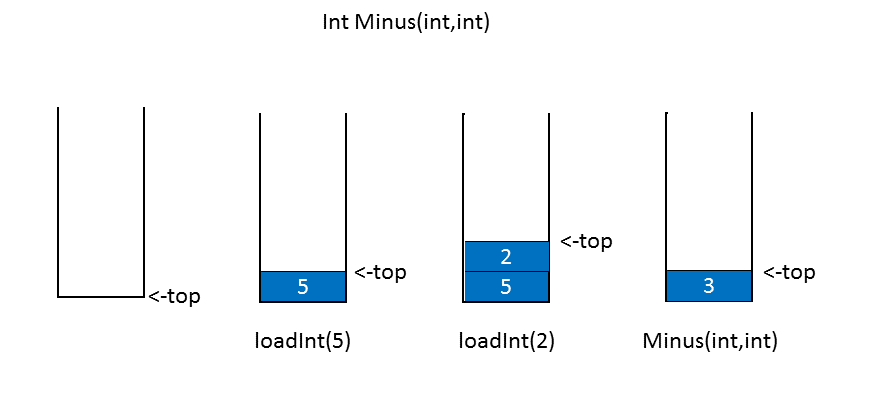
\includegraphics[scale=0.5]{images/BeispielStack.png}
\caption{Beispiel einer Minus Operation mit den Parametern (5,2)}
\label{example_stack}
\end{figure}
Eine Instruktion im MSIL Code setzt sich jeweils aus einem OpCode und einem Operand zusammen.
\begin{lstlisting}
ldsflda    class TestProgram.NewObject TestProgram.Program::_obj1
\end{lstlisting}
In diesem Beispiel eines IL Code ist "ldsflda" der OpCode und "class TestProgram.NewObject TestProgram.Program::\_obj1" der Operand. Der OpCode (Operation Code) identifiziert was die Operation durchführen soll. Hier "ldsflda" (Load Static Field Address). Dabei wird vom Operand definierten Static Field die Speicheradresse ausgelesen und auf den Stack gelegt. Der Operand ist daher jeweils die Ressource welche für den OpCode verwendet wird. Der Typ des Operand ist durch den OpCode definiert.\\
Um erfolgreich den Source Code für den Dynamic Parallel Checker zu instrumentieren (sh. \autoref{example_injection}), muss der Aufbau des Stacks immer sichergestellt werden. Daher müssen Werte um Sie aus dem Stack herauszulesen, immer dupliziert werden, damit das Programm erfolgreich durchgeführt werden kann.\\
\begin{figure}[H]
\centering
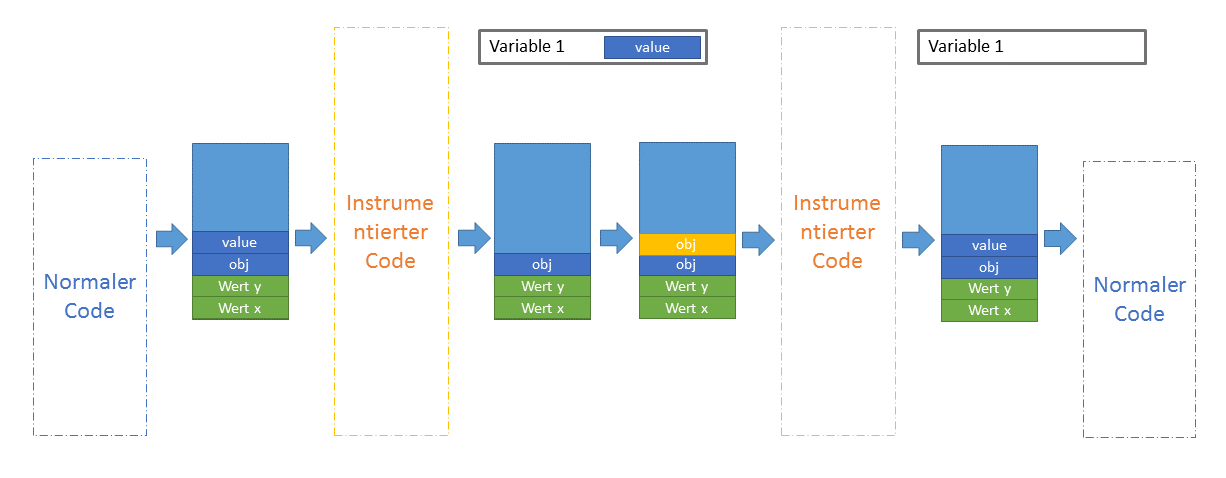
\includegraphics[scale=0.5]{images/BeispielInjection.png}
\caption{Beispiel Code Injection, Stack verhalten}
\label{example_injection}
\end{figure}
In \autoref{example_injection} ist ein Beispiel dargestellt, wie eine Injection den Stack verwaltet und dabei die benötigte Information "obj" aus dem Stack extrahiert und den Ursprungszustand wiederherstellt. Da bei einem LIFO Stack nur auf das oberste Element zugegriffen werden kann, wird der Top-Wert "value" in eine lokale Variable gespeichert. Nach dem Abbau des duplizieren "obj" wird der Wert wieder aus der Variable auf den Stack gelegt.
\end{flushleft}
\subsection{Implementation}\label{implementation}
In diesem Kapitel wird die Implementation des Dynamic Prallel Checker genauer erklärt. Unter \ref{example} ist das Beispiel beschrieben an welchem, in den folgenden Kapitel, die Funktion des Dynamic Parallel Checkers beschrieben wird. Der Dynamic Parallel Checker wurde mit C\#.Net entwickelt.
\newpage
\subsubsection{Beispiel}\label{example}
\begin{flushleft}
Der Vektor Clock Algorithmus wird in diesem Kapitel mit Hilfe von folgendem Pseudo-Code Beispiel genauer erläutert.\\
\begin{figure}[H]
\begin{singlespace}
\begin{lstlisting}
//... Deklaration a,b,locka,lockb...

Thread.Start(() =>		// start thread2 (T2)
{
	lock(lockb) {
		b = 3;
	}
	b = 4;
	lock(locka) {
		Console.WriteLine(a);
	}
});
Thread.Start(() =>		// start thread3 (T3)
{
	lock(locka) {
		a = 2;
	}
	b = 5;
	lock(lockb) {
		Console.WriteLine(b);
	}
})
lock(locka) {
	a = 3;
}
lock(lockb) {
	b = 6;
}
Console.WriteLine(a);
\end{lstlisting}
\end{singlespace}
\caption{Beispiel für die Erklärung des Algorithmus}\label{basic_example}
\end{figure}
Da der Code in \autoref{basic_example} asynchron durchgeführt wird, werden die 3 enstehenden Thread parallel ausgeführt und es kann das Muster aus \autoref{basic_example_parallel} entstehen.
\begin{figure}[H]
\centering
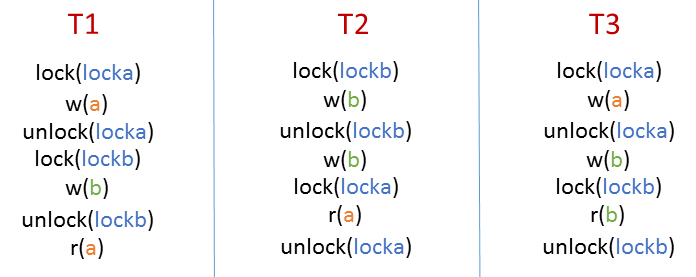
\includegraphics[scale=0.5]{images/VectorCheckingAlgorithm.png}
\caption{Darstellung der parallelen Vorgänge von \autoref{basic_example}}
\label{basic_example_parallel}
\end{figure}
\end{flushleft}
\newpage
\subsubsection{Vector Clock pro Thread}
\begin{flushleft}
Die Vector Clock eignet sich optimal for die History des Dynamic Parallel Checkers. Jeder Thread erhält seine eigene Vektor Clock, in der er die Zeitstempel der anderen Threads mitführt. Es wird nicht der aktuelle Zeitstempel mitgeführt, sondern der Zeitstempel der bei der letzten direkten oder indirekten Synchronisation mit diesem Thread von diesem Thread mitgeliefert wurde. Bei einem Synchronisationspunkt wird die Vector Clock mit der Vector Clock aus der Lock-History synchronisiert. (sh. \ref{lock_history}) Die Reihenfolge der Synchronisation ist jedoch nicht deterministisch und hängt vom Scheduler ab.\\
Unser Algorithmus verwendet die Vector Clock des aktuellen Threads um diese mit den Vector Clocks der History der anderen Threads zu vergleichen, um herauszufinden welche Zugriffe neben läufig zu dem aktuellen Zugriff stattgefunden haben. Daher ist es sehr wichtig, dass jeder Thread seine eigene Vector Clock hat.
\end{flushleft}
\subsubsection{Lock-History}\label{lock_history}
\begin{flushleft}
Während der kompletten Überwachung wird eine Lock-History geführt. Diese beinhaltet die Information welcher Thread auf welche Ressource zu welcher Zeit (Vector Clock) einen Lock durchgeführt hat. Diese Information wird benötigt um z.B. eine Synchronisation zwischen dem Thread, der den letzten Unlock auf eine Ressource durchgeführt hat, mit dem aktuellen Thread, der nun einen Lock auf die selbe Ressource durchführen möchte, vorzunehmen. Bei jedem Unlock wird ein neuer Lock-History Eintrag erstellt, falls noch keiner vorhanden ist. Sollte jedoch bereits einer vorhanden sein, wird dieser überschrieben. Eine Lock-History könnte wie folgt aussehen:\\
\end{flushleft}
\begin{center}
\textbf{\textit{Lock-History:}}\\[0.5cm]
\begin{tabular}{ c c c }
  Vektor & Ressource & ThreadNr \\\hline
  (1,1,0) & locka & 2 \\
  (1,0,0) & lockb & 1 \\\hline\\
\end{tabular}
\end{center}
\textbf{Synchronisation der Vektor Clock}
\begin{flushleft}
Wenn z.B. in unserem Beispielprogramm Thread1 (T1) vor Thread3 (T3) in den Lock(a) Bereich kommt, schreibt er beim Verlassen des gesicherten Bereichs einen Eintrag in die Lock-History. Wenn nun T3 de Lock(a) beziehen möchte, sieht der Algorithmus zuerst in die Lock-History ud synchronisiert seine Vector Clock ()

TODO: Beispiel umschreiben\\
Wenn z.B. in unserem Beispielprogramm Thread1(T1) vor Thread3(T3) in den lock(a) Bereich kommt, schreibt er beim Verlassen des gesicherten Bereichs einen Eintrag in die Lock-History. Wenn nun T3 den lock von a beziehen möchte schaut er zuerst in die Lock-History und synchronisiert seine Vektor Clock (a1,a2,a3) mit der Vektor Clock des Eintrags in der Tabelle (b1,b2,b3).\\
Die neue Vektor Clock von T3 lässt sich nun wie folgt bilden: 
\begin{center}(b1, max(a2, b2), a3 + 1)\end{center}
\textit{Erklärung:}
\begin{itemize}
\item Von dem Thread, dessen Eintrag in der Lock-History zu einer Synchronisation führte, kann direkt der Wert übernommen werden.
\item Der synchronisierende Thread kann den eigenen Wert übernehmen und die Zahl 1 addieren.
\item Von jedem Thread der nicht in die Synchronisation involviert ist kann max(a, b) genommen werden.
\end{itemize}
Nach der Synchronisation ist eine Barriere aufgebaut. Kein Ereignis von T3 kann nach der Synchronisation mit einem Ereignis von T1 vor der Synchronisation in Konflikt stehen.
\end{flushleft}
\subsubsection{Vector Clock Algorithmus}\label{vector_algorithm}
\textbf{Vector Clock Management Algorithmus}
\begin{flushleft}

\end{flushleft}
\textbf{Algorithmus Beispiel}
\begin{flushleft}
TODO: Wir werden nun den Beispiel Code durchspielen und dabei die Lock-History befüllen:\\
\begin{itemize}
\item Wenn alle Threads gestartet sind.\\[0.3cm]
\begin{tabular}{ c c c }
  	Vektor & Ressource & ThreadNr \\\hline
  	  &   &   \\\hline
\end{tabular}
\[
	T1 = \begin{pmatrix}
		T1 & 1\\
	\end{pmatrix}
	, T2 = \begin{pmatrix}
		T2 & 1\\
	\end{pmatrix}
	, T3 = \begin{pmatrix}
		T3 & 1\\
	\end{pmatrix}
\]
\item lock(lockb) von Thread2\\[0.3cm]
\begin{tabular}{ c c c }
  	Vektor & Ressource & ThreadNr \\\hline
  	(,1,0) & lockb & 2 \\\hline
\end{tabular}
\[
	T1 = \begin{pmatrix}
		T1 & 2\\
		T2 & 0\\
		T3 & 3\\
	\end{pmatrix}
	, T2 = \begin{pmatrix}
		T1 & 2\\
		T2 & 0\\
		T3 & 3\\
	\end{pmatrix}
	, T3 = \begin{pmatrix}
		T1 & 2\\
		T2 & 0\\
		T3 & 3\\
	\end{pmatrix}
\]
\end{itemize}
\end{flushleft}

\textbf{Race Condition Check}
\begin{flushleft}

\end{flushleft}
\subsubsection{Instrumentation}
\begin{flushleft}
Für die Durchführung des Vector Clock Algorithmus (sh. Kapitel \ref{vector_algorithm}) ist es wichtig die Informationen über Lese- / Schreibzugriffe sowie Locks und Thread.Starts zu erhalten. Dazu muss der bestehende IL Code angepasst (instrumentiert) werden, damit er diese Informationen preisgibt. Dazu wird der Code analysiert und an Stellen mit wichtigen Zugriffen um Code erweitert. Wie in Kapitel \ref{chapter_IL} bereits beschrieben muss dabei der korrekte Aufbau des Stack jederzeit sichergestellt werden. Für die Instrumentation des Codes wird die Library Mono.Cecil aus dem Mono Projekt verwendet. Die Library erlaubt es den IL Code zu lesen und zu bearbeiten. 
\begin{figure}[H]
\centering
\begin{lstlisting}[language=CIL,backgroundcolor=\color{backcolor}]
IL_001a:  box        [mscorlib]System.Int32
IL_001f:  stsfld     object TestProgram.Program::_a
\end{lstlisting}
\caption{Beispiel ohne Instrumentation}\label{example_codeWithoutInstrum}
\end{figure}
\autoref{example_codeWithoutInstrum} zeigt ein Beispiel, eines typischen Schreibzugriff im MS IL. Der Befehl "box" führt ein Boxing eines Integers durch. Dabei wird der Integerwert von einem Valuetype zu einem Referenztyp umgebaut. Auf dem Stack liegt nach dem Boxing die Adresse des Integer-Werts. Diese Adresse wird dann verwendet um den Wert in die Variable "\_a" mit dem Befehl "stsfld"(Store Static Field) zu speichern.\\
\begin{figure}[H]
\centering
\begin{lstlisting}[language=CIL,backgroundcolor=\color{backcolor}]
IL_001a:  box        [mscorlib]System.Int32
//----------Instrumented Code...----------------
IL_001f:  ldsflda    object TestProgram.Program::_a
IL_0024:  ldc.i4.s   31
IL_0026:  ldstr      "System.Void TestProgram.Program::Test()"
IL_002b:  call       void [DPCLibrary]DPCLibrary.DpcLibrary::
                                 WriteAccess(int32,int32,string)
//----------...End Instrumentation--------------
IL_0030:  stsfld     object TestProgram.Program::_a
\end{lstlisting}
\caption{Instrumentierter IL Code}\label{example_instrumentedCode}
\end{figure}
\autoref{example_instrumentedCode} zeigt den Code nach dem der Dynamic Parallel Checker diesen instrumentiert hat. Wie in \autoref{example_codeWithoutInstrum}, startet der Code mit "box" und endet mit "stsfld". Dazwischen wurde der Code um den Dynamic Parallel Checker erweitert. Um zu wissen auf welche Variable der Schreibzugriff durchgeführt wird, wird mit "ldsflda" (Load static Field Address) die Adresse der Resource ausgelesen und auf den Stack gelegt. Danach wird die Zeilennummer des Schreibzugriff auf den Stack gelegt (Man beachte: Die Zeilennummer zeigt die Zeile vor der Instrumentation) um bei einem Fehler aufzuzeigen, welche Code Zeilen diesen verursacht haben. Daher wird auch als nächstes der Methodennamen als String auf den Stack gelegt. Als letzte instrumentierte Zeile werden dann die Informationen an den Dynamic Parallel Checker übergeben. Dies wird mit der Methode "WriteAccess(int32,int32,string)" durchgeführt. Nach dem Instrumentierten Code hat der Stack wieder den gleichen Zustand wie nach dem "Box" Befehl in \autoref{example_codeWithoutInstrum}.
\end{flushleft}
\subsection{Schlussfolgerungen}
TODO
\subsubsection{Technische Findings}
TODO\\
-Task/Threads
\subsubsection{Persönliches Fazit}
TODO
\subsection{Backlog}
TODO
\section{Glossar}
- Partielle Ordnung\\
- Totale Ordnung
\section{Abbildungsverzeichnis}
\listoffigures
\section{Literaturverzeichnis}
\renewcommand{\section}[2]{}%
\begin{thebibliography}{xxxxxxxxxxxxx}
\bibitem[BMBF, 2003]{bmbf}"'IT-Ausstattung der allgemein bildenden und berufsbildenden 
                         Schulen in Deutschland"', http://www.schulen-ans-netz.de/   
                         neuemedien/fakten/dokus/it-ausstattung-2003.pdf, 10.03.2005	
\bibitem[ECMA, 2012]{ecma}"Standard ECMA-335 Common Language Infrastructure (CLI)", http://www.ecma-international.org/publications/standards/Ecma-335.htm, 06.2012
\end{thebibliography}
\end{document}
